\chapter{Projeto - Parte 4}\label{ch:projeto-parte4}

TODO()


\section{Arquitetura Deliberativa}\label{sec:arquitetura-deliberativa}

Conforme foi abordado na secção~\ref{sec:arquiteturas-reativa-memoria}, um agente reativo com memória age com conhecimento do presente, através de reações a estímulos, e com conhecimento do passado, através da memorização de percepções e de ações passadas.
Um agente deliberativo, além de possuir as características de um agente reativo com memória, é capaz de antecipar o futuro, através da simulação de cenários, e consequentemente de planear ações futuras, com base em objetivos explícitos (fixos ou gerados dinamicamente) e em processos de deliberação sobre que objetivos concretizar e quais os meios a utilizar.

Qualquer sistema para poder antecipar o futuro tem que ter conhecimento (modelo do mundo), e esse conhecimento pode ser adquirido através da experiência ou de algo que já tenha esse conhecimento e o transmita para o agente (e.g., num ambiente multi-agente, um agente pode adquirir conhecimento de outro agente).
O modelo do mundo caracteriza-se como um caso particular da representação do modelo do problema, e permite simular para cada opção as múltiplas sequências de evolução possíveis, através de uma simulação interna (sequência de ações)~\cite{isel:iasa:slides:arq-agentes-deliberativos}.

A sequência de ações geradas por um agente deliberativo, através de processos internos, caracterizam o seu comportamento, ao contrário dos agentes reativos que têm comportamentos baseados em reações.

Numa arquitetura deliberativa, o módulo de memória é indispensável e dá suporte à simulação interna e aos mecanismos de deliberação~\cite{isel:iasa:slides:arq-agentes-deliberativos}, conforme representado na figura~\ref{fig:arquitetura-deliberativa}.

\begin{figure}[H]
    \begin{center}
        \resizebox{100mm}{!}{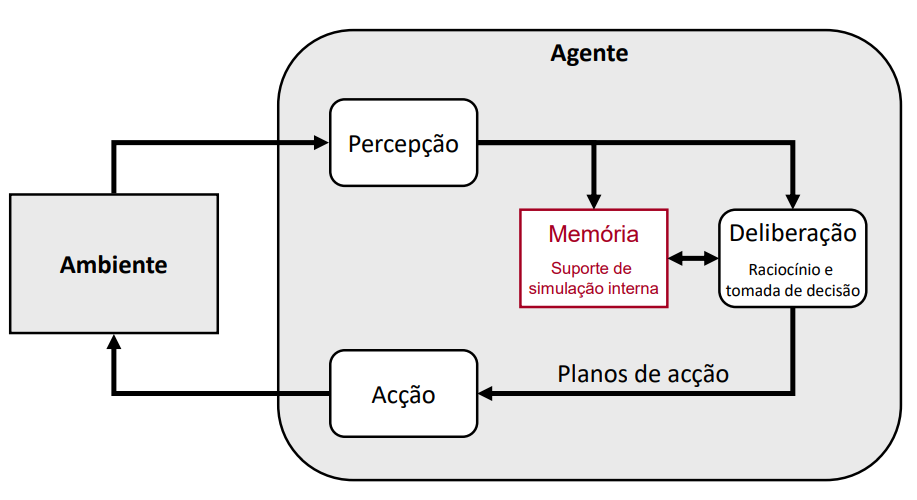
\includegraphics{../figures/arquitetura-deliberativa}}
    \end{center}
    \caption{Arquitetura deliberativa.
    Retirado de~\cite{isel:iasa:slides:arq-agentes-deliberativos}, slide 16.}
    \label{fig:arquitetura-deliberativa}
\end{figure}


\section{Raciocínio Automático}\label{sec:raciocinio-automatico-1}

Conforme foi abordado na secção~\ref{sec:raciocinio-automatico}, o raciocínio automático é um processo de inferência que permite a um agente deliberativo deduzir novas informações a partir de conhecimento prévio.

Com base nos conhecimentos adquiridos nesta fase do projeto, este raciocínio pode ser subdividido em dois tipos:

\begin{itemize}
    \item \textbf{Raciocínio Prático}: orientado para a ação (interação permanente com o mundo, ao qual está associado o processo de tomada de decisão).
    Tem como input os objetivos a atingir, as ações realizáveis e a representação do mundo, e como output os planos de ação.
    \item \textbf{Raciocínio Teórico}: orientado para o conhecimento, que permite deduzir novas informações a partir de conhecimento prévio.
    Caracteriza-se por ser direto, ou seja, não envolve interação com o mundo.
\end{itemize}

\subsection{Raciocínio Prático}\label{subsec:raciocinio-pratico}

Numa arquitectura deliberativa, o raciocínio prático suporta o processo
geral de tomada de decisão que determina o comportamento do agente,
ou seja, quais as acções a realizar perante as percepções obtidas e o
estado do modelo interno do mundo~\cite{isel:iasa:slides:arq-agentes-deliberativos}.
Este processo de tomada de decisão é composto por duas fases:

\begin{itemize}
    \item \textbf{Deliberação}: raciocínio sobre os fins, que permite definir os objetivos a atingir (i.e., opções (input) -> objetivos (output)).
    \item \textbf{Planeamento}: raciocínio sobre os meios, que permite definir os planos de ação a executar (i.e., ações (input) -> planos (output)).
\end{itemize}

Tendo em conta que o raciocínio prático é um processo de tomada de decisão, é necessário que o agente tenha objetivos, que são os critérios de avaliação das ações, e que possa avaliar as ações possíveis, de forma a escolher a melhor ação a executar.
Portanto, a deliberação sobre a representação do modelo do mundo que permite definir os objetivos, e o planeamento com base nesses e nos meios disponíveis, definem os processos necessários para a geração de planos de ação, conforme representado na figura~\ref{fig:delib-planeamento}.

\begin{figure}[H]
    \begin{center}
        \resizebox{100mm}{!}{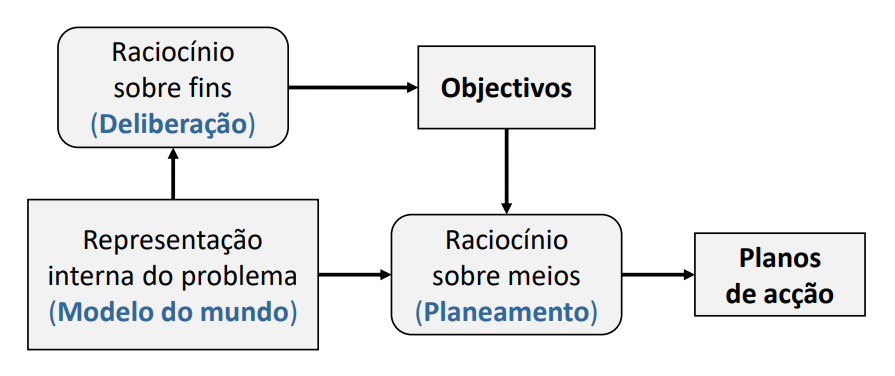
\includegraphics{../figures/delib-planeamento}}
    \end{center}
    \caption{Deliberação e planeamento num agente deliberativo.
    Retirado de~\cite{isel:iasa:slides:arq-agentes-deliberativos}, slide 8.}
    \label{fig:delib-planeamento}
\end{figure}

No entanto, o ambiente pode ser dinâmico, e por isso o agente pode ter que reagir a mudanças no ambiente (i.e., alterações no modelo do mundo), o que implica que o processo de tomada de decisão seja adaptativo, ou seja, que possa ser reavaliado e ajustado (reconsideração).
Além disso, mesmo sem alteração do estado do ambiente, o próprio plano de ação pode alterar-se ao longo do tempo e estar desfasado da realidade, devido a um acontecimento que não foi antecipado (e.g., um camião que seguia um trajeto específico, mas por causa de areia no caminho, teve que mudar de trajeto).

Portanto, o processo geral de tomada de decisão, que ocorre de forma cíclica, pode ser então representado pelos seguintes passos~\cite{isel:iasa:slides:arq-agentes-deliberativos}:

\begin{enumerate}
    \item Observar o mundo, gerando percepções.
    \item Atualizar o modelo do mundo, com base nas percepções.
    \item Se reconsiderar, então:
    \begin{enumerate}
        \item Deliberar o que fazer, gerando um conjunto de objetivos.
        \item Planear como fazer, gerando um plano de ação.
    \end{enumerate}
    \item Executar o plano de ação.
\end{enumerate}

\subsection{Racionalidade Limitada}\label{subsec:racionalidade-limitada}

A racionalidade limitada é um conceito que se aplica a agentes que têm recursos computacionais limitados (i.e., tempo de computação, memória), e que por isso não conseguem gerar planos de ação ótimos.

Portanto, um agente com racionalidade limitada tenta chegar a uma solução satisfatória, não à melhor solução, de forma dinâmica, tendo em conta os recursos computacionais disponíveis.
Divide o problema em subproblemas mais simples, e resolve-os sequencialmente, de forma a atingir o objetivo final.


\section{Implementação do Agente Deliberativo}\label{sec:implementacao-agente-deliberativo}
